%        File: 03140299.tex
%     Created: Fri Jan 02 03:00 PM 2015 J
% Last Change: Fri Jan 02 03:00 PM 2015 J
%
\documentclass[10pt,a4paper,twocolumn]{jarticle}

%%%%%%%%%%%%%%%%%%%%%
% to input Japanese %
%%%%%%%%%%%%%%%%%%%%%
\usepackage[japanese]{babel}

%%%%%%%%%%%%%%%%%%%%%
% to insert itembox %
%%%%%%%%%%%%%%%%%%%%%
\usepackage{ascmac}

%%%%%%%%%%%%%%%%%%%%%%%%%%
% to be standard a4paper %
%%%%%%%%%%%%%%%%%%%%%%%%%%
\usepackage{geometry}
\geometry{
  a4paper,
  total={210mm,297mm},
  left=20mm,
  right=20mm,
  top=20mm,
  bottom=40mm,
}

%%%%%%%%%%%%%%%%%%%%%
% to insert figures %
%%%%%%%%%%%%%%%%%%%%%
\usepackage[dvipdfmx]{graphicx}

%%%%%%%%%%%%%%%%%%%%%%%%%%
% to insert source codes %
%%%%%%%%%%%%%%%%%%%%%%%%%%
% \usepackage{listings, jlisting}
% \renewcommand{\lstlistingname}{list}
% \lstset{language=C,
%   basicstyle=\ttfamily\scriptsize,
%   commentstyle=\textit,
%   classoffset=1,
%   keywordstyle=\bfseries,
%   frame=tRBl,
%   framesep=5pt,
%   showstringspaces=false,
%   numbers=left,
%   stepnumber=1,
%   numberstyle=\tiny,
%   tabsize=2
% }

%%%%%%%%%%%%%%%%%%
% title & author %
%%%%%%%%%%%%%%%%%%
\title{ロボットインテリジェンス レポート課題A \\
      「ニューラルネット学習シミュレーション」}
\author{03-140299 東京大学機械情報工学科3年 和田健太郎}

%%%%%%%%%%%%%%%%%%
% begin document %
%%%%%%%%%%%%%%%%%%
\begin{document}
\maketitle

%%%%%%%%%%%%%%%%%%%%%%%%%%%%%%%%%%%%%%%%%%%%%%%%%%%%%%%%
\section{はじめに}
レポート課題として課題Aを選択し, 3層フィードフォワード型の
ニューラルネットとバックプロパゲーション学習をシミュレーション
するプログラムを作成し, 識別実験を行った. 
実験に利用したデータ群は
The MNIST database of handwritten digits
であり, このデータは過去に様々な分類器において
識別能力を図るために利用されている. \cite{mnist}
図\ref{fig:plot-mnist}に実際に利用した学習データの一部を示す. 
\begin{figure}[htbp]
  \centering
  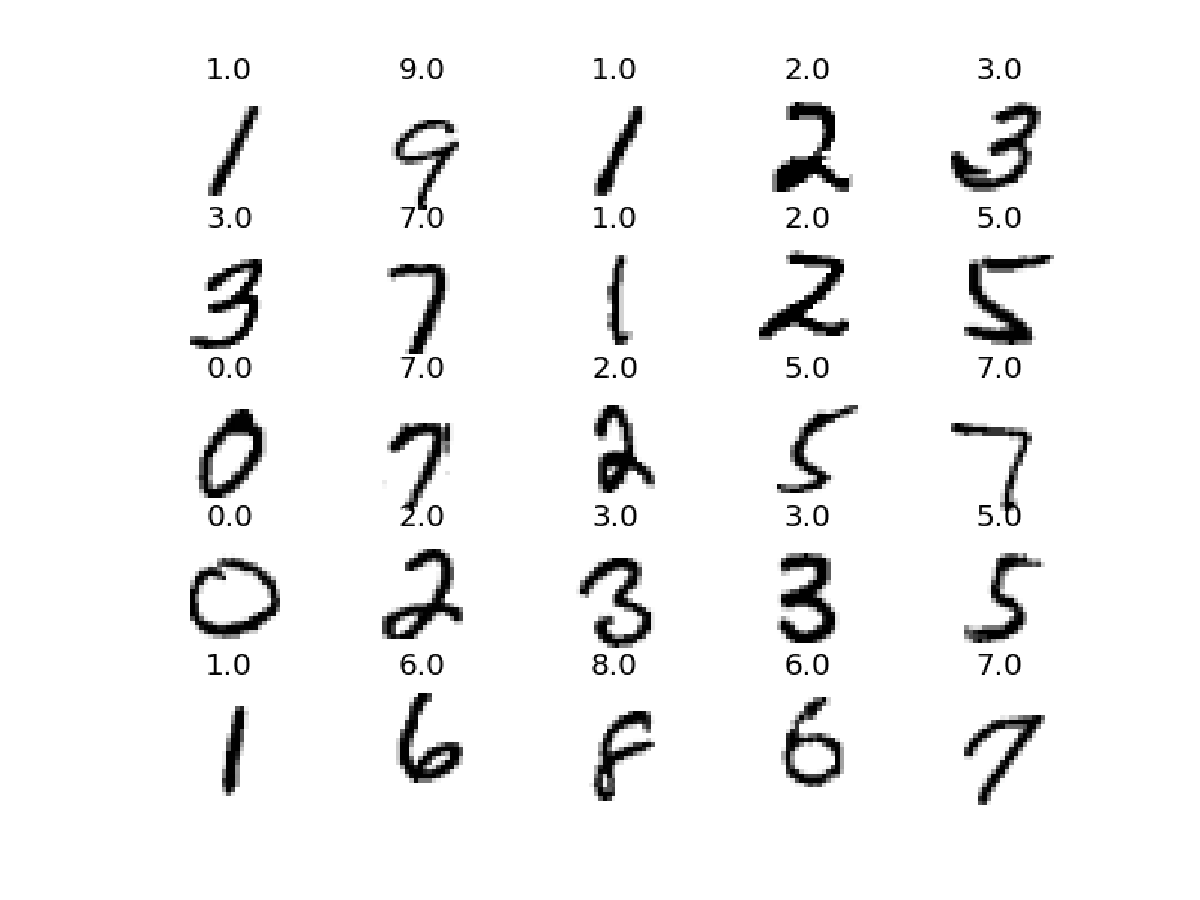
\includegraphics[width=0.4\textwidth]{assets/img/plot_mnist.pdf}
  \caption{MNISTの画像データ例}
  \label{fig:plot-mnist}
\end{figure}

また, ノイズを加えた場合の性能変化, ノイズ耐性, 
中間ニューロンの役割, オートエンコーダを利用した画像特徴抽出による
識別性能変化について考察した. 
%%%%%%%%%%%%%%%%%%%%%%%%%%%%%%%%%%%%%%%%%%%%%%%%%%%%%%%%

%%%%%%%%%%%%%%%%%%%%%%%%%%%%%%%%%%%%%%%%%%%%%%%%%%%%%%%%
\section{ニューラルネット学習シミュレーション}
実験に利用したMNISTデータセットは, 28x28のグレースケールの手書き数字
画像データである. 画像に対する前処理はなしで7000件のデータに対して,
学習率と慣性項係数のそれぞれに関して複数の値を用いて識別正解率の変化を調べた. 

慣性項は0に固定して, 学習率を0.02から0.38まで0.02ずつ変化させ,
学習率と識別正解率の関係を表したのが
図\ref{fig:learning-rate-score-var}である. 
図から, 学習率が0.3のときに最も識別正解率が高いことがわかる. 

学習率を0.3に固定して, 慣性項の係数を0.0から0.38まで変化させ,
慣性項係数と識別正解率の関係を表したのが
図\ref{fig:inertia-rate-score-var}である. 
\begin{figure}[htbp]
  \centering
  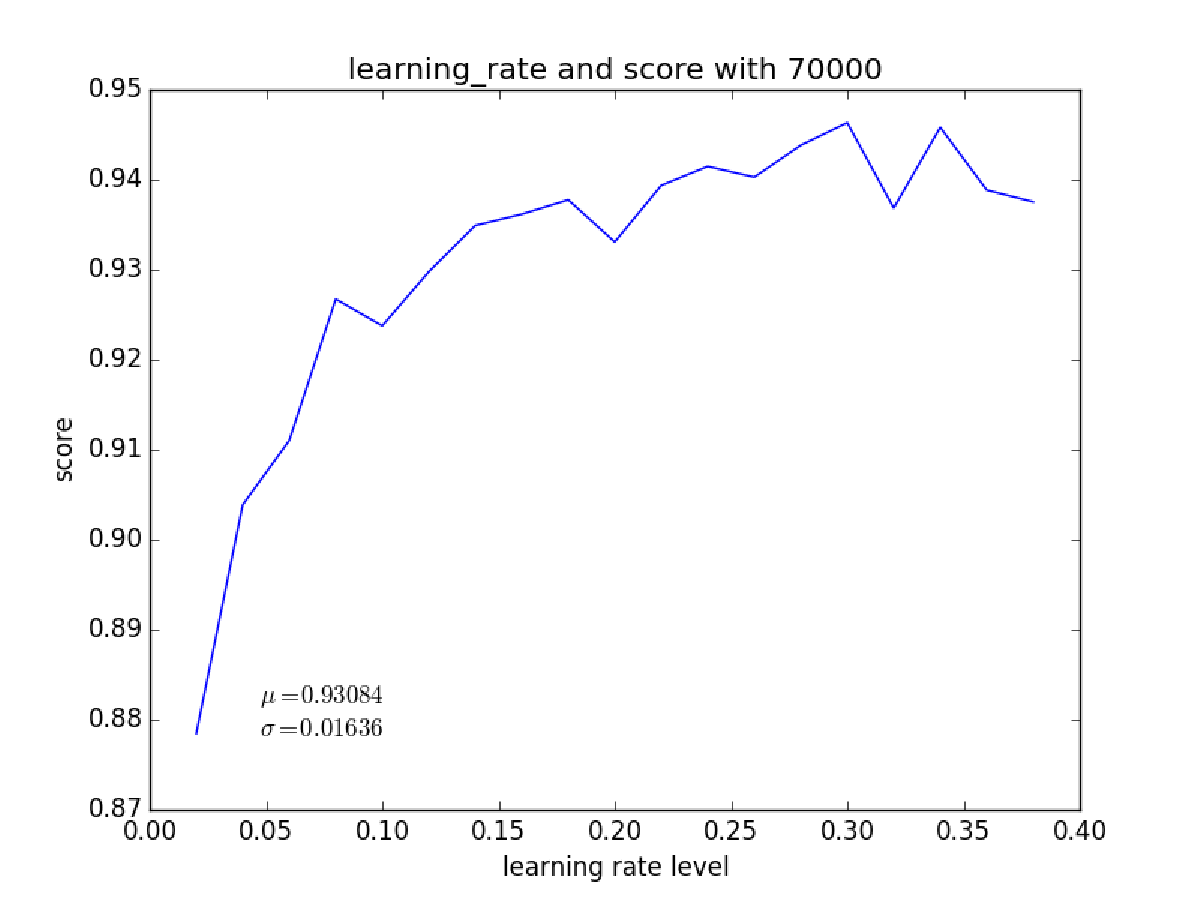
\includegraphics[width=0.4\textwidth]{assets/img/learning_rate_test_mnist_70000.pdf}
  \caption{学習率と識別正解率の関係}
  \label{fig:learning-rate-score-var}
\end{figure}
\begin{figure}[htbp] 
  \centering
  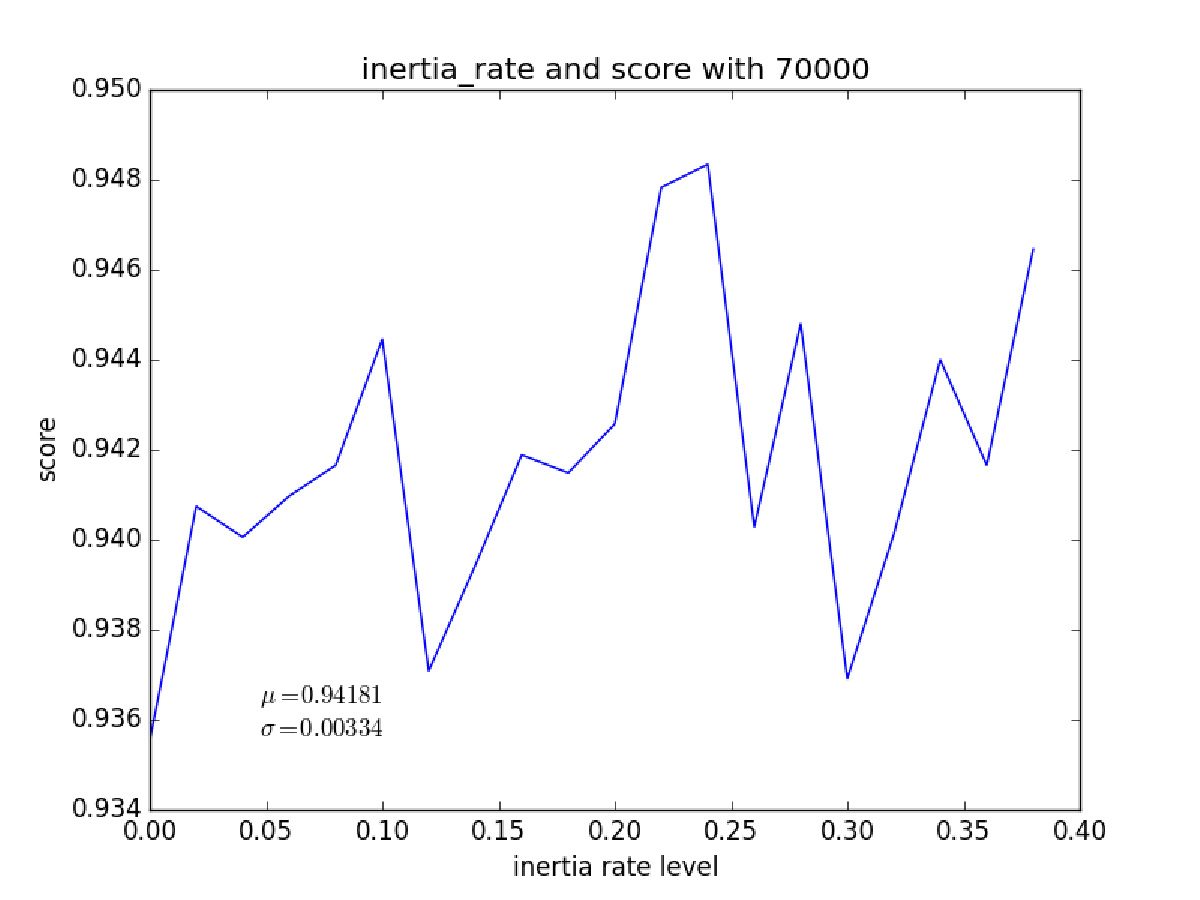
\includegraphics[width=0.4\textwidth]{assets/img/inertia_rate_test_mnist_70000.pdf}
  \caption{慣性項の係数と識別正解率の関係}
  \label{fig:inertia-rate-score-var}
\end{figure}

今後の解析では学習率を0.3, 慣性項の係数を0.24として実験を行う.
%%%%%%%%%%%%%%%%%%%%%%%%%%%%%%%%%%%%%%%%%%%%%%%%%%%%%%%%

%%%%%%%%%%%%%%%%%%%%%%%%%%%%%%%%%%%%%%%%%%%%%%%%%%%%%%%%
\section{ノイズによる性能変化}
ノイズによる識別性能の変化について検証した. 
ノイズは, ある確率で画像のピクセル値を
ランダムな値に変化させるということで発生させた. 
図\ref{fig:noise-test-score-var-10000}, 
\ref{fig:noise-test-score-var-70000}
はノイズの発生する確率と識別性能の関係を表した図である. 
データは10000件(図\ref{fig:noise-test-score-var-10000})と
70000件(図\ref{fig:noise-test-score-var-70000}), 
ノイズの発生確率は0.0から0.25まで0.01ずつ変化させた. 
図より, ノイズの確率0.04のとき識別正解率が最も高くなっていることがわかる. 

また, 10000サンプルの場合には正解率の平均が0.85721, 標準偏差が0.04707であり, 
70000サンプルでは平均0.94010, 標準偏差0.00332であることから
ノイズ耐性はデータ数によって上がると言える. 
\begin{figure}[htbp] 
  \centering
  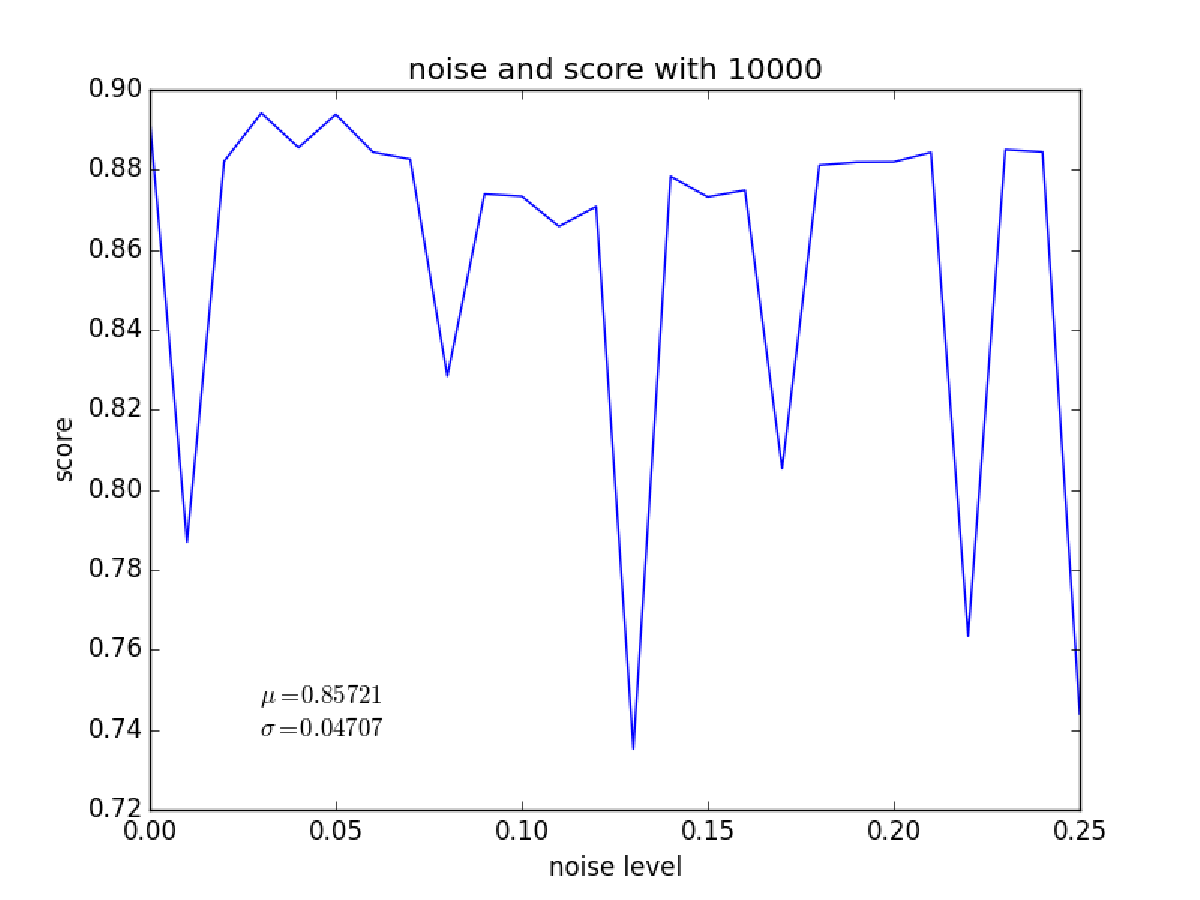
\includegraphics[width=0.4\textwidth]{assets/img/noise_test_mnist_10000.pdf}
  \caption{ノイズと識別正解率の関係(10000サンプル)}
  \label{fig:noise-test-score-var-10000}
\end{figure}
\begin{figure}[htbp] 
  \centering
  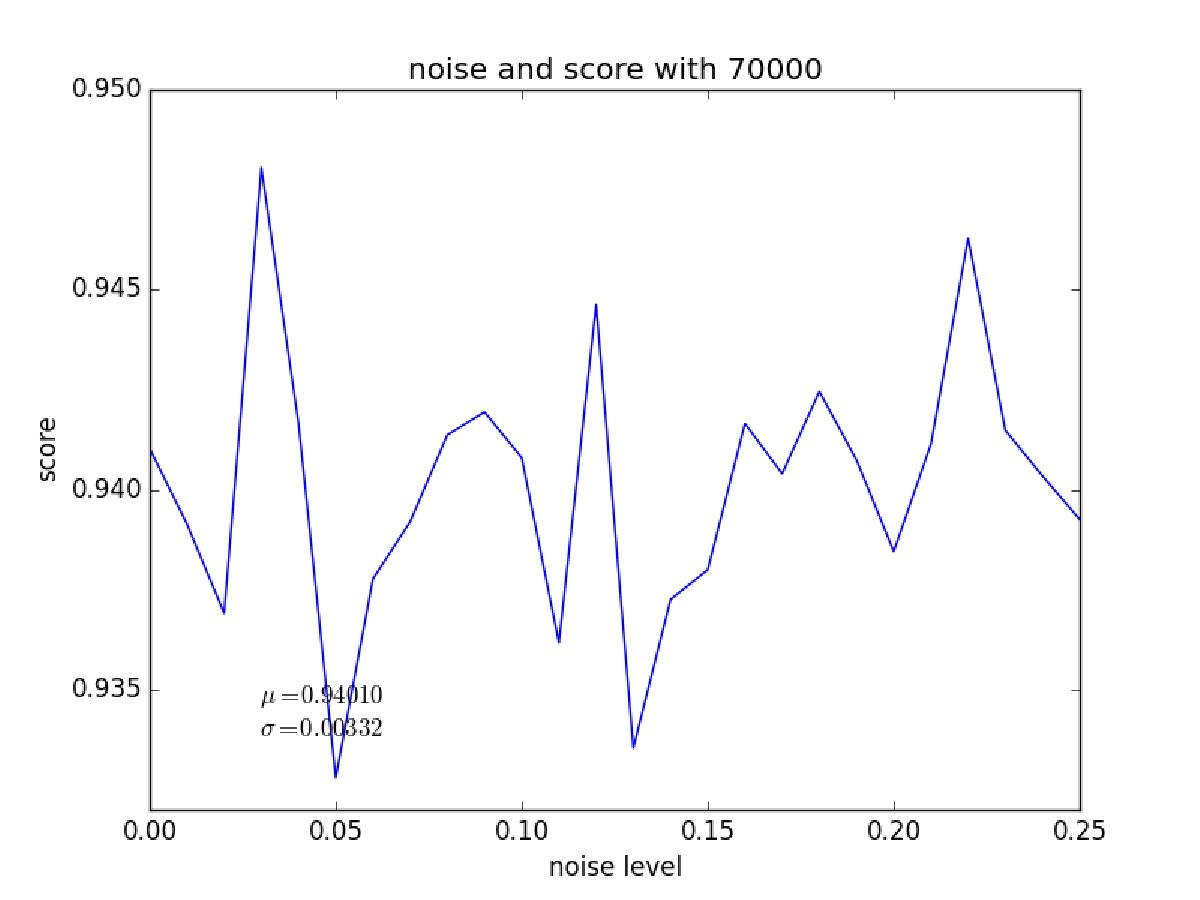
\includegraphics[width=0.4\textwidth]{assets/img/noise_test_mnist_70000.pdf}
  \caption{ノイズと識別正解率の関係(70000サンプル)}
  \label{fig:noise-test-score-var-70000}
\end{figure}
%%%%%%%%%%%%%%%%%%%%%%%%%%%%%%%%%%%%%%%%%%%%%%%%%%%%%%%%

%%%%%%%%%%%%%%%%%%%%%%%%%%%%%%%%%%%%%%%%%%%%%%%%%%%%%%%%
\section{中間層のニューロンの役割}
中間層のニューロンの数を変化させ, ニューロン数と識別性能の関係を表した
のが図\ref{fig:hidden-neuron-role}である. 
\begin{figure}[htbp]
  \centering
  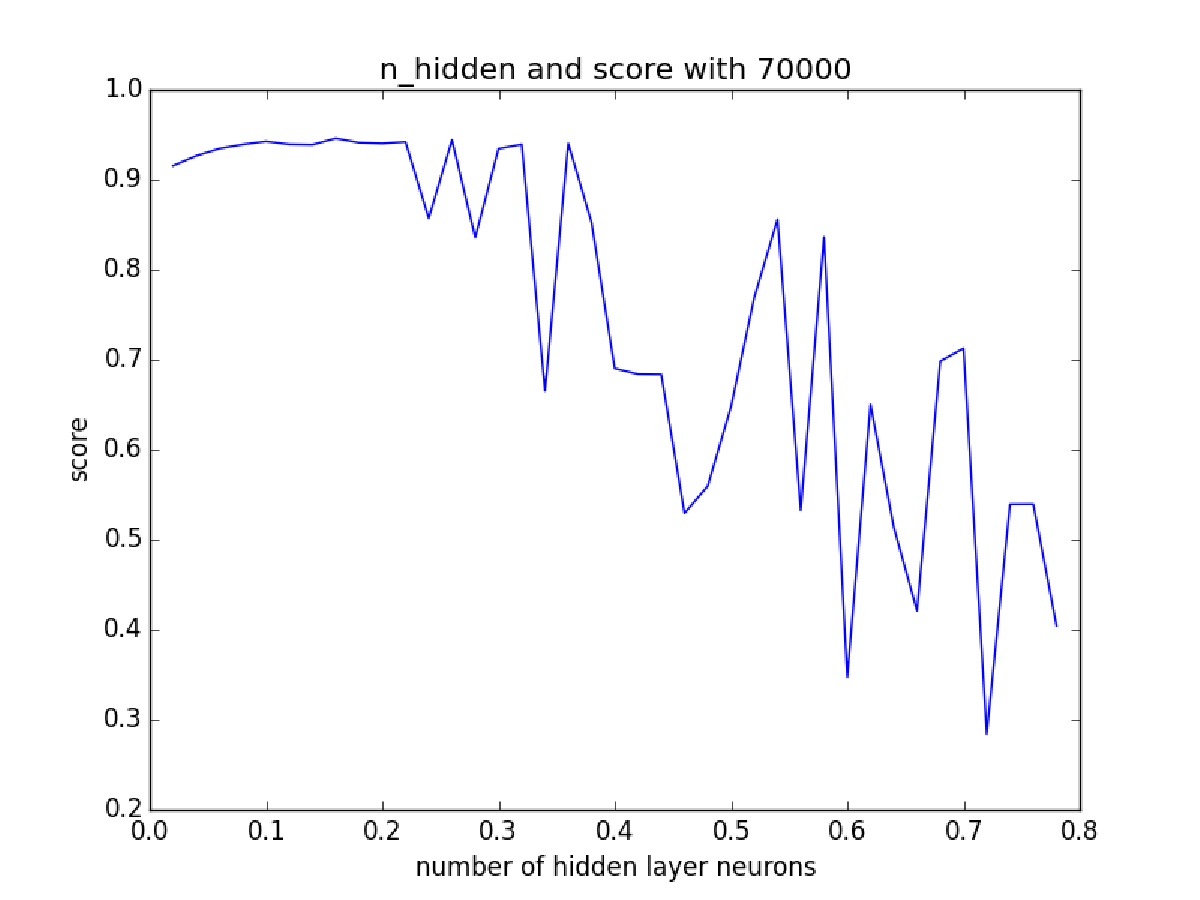
\includegraphics[width=0.4\textwidth]{assets/img/hidden_layer_analyze_mnist_score_70000.pdf}
  \caption{中間層ニューロン数と識別器の識別性能の関係}
  \label{fig:hidden-neuron-role}
\end{figure}

\begin{figure}[htbp] 
  \centering
  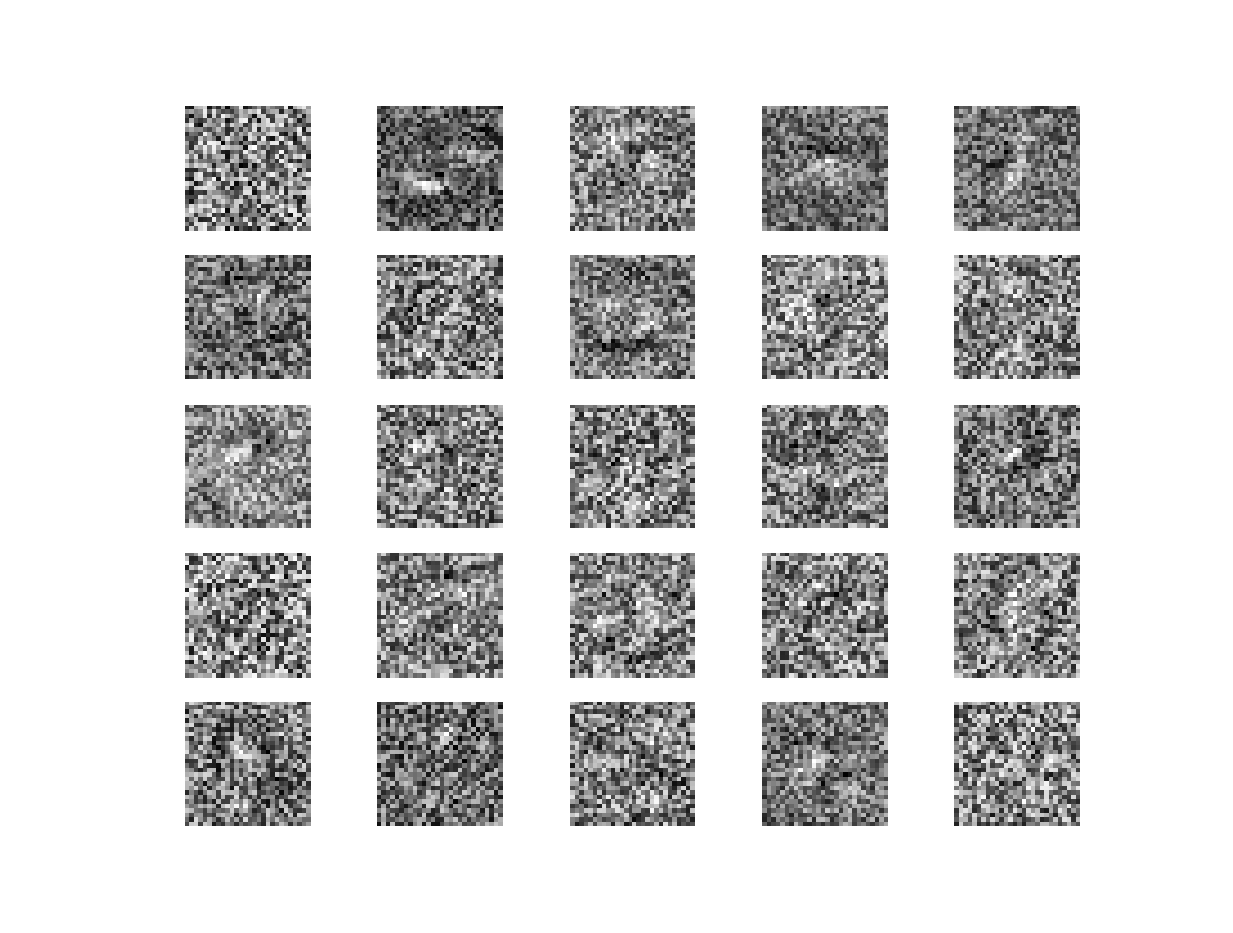
\includegraphics[width=0.4\textwidth]{assets/img/hidden_layer_analyze_mnist_image_nsamp70000_nh0.16.eps}
  \caption{識別性能が高い場合(中間層0.16)の重み}
  \label{fig:hidden-layer-analyze-img-0.16}
\end{figure}
\begin{figure}[htbp] 
  \centering
  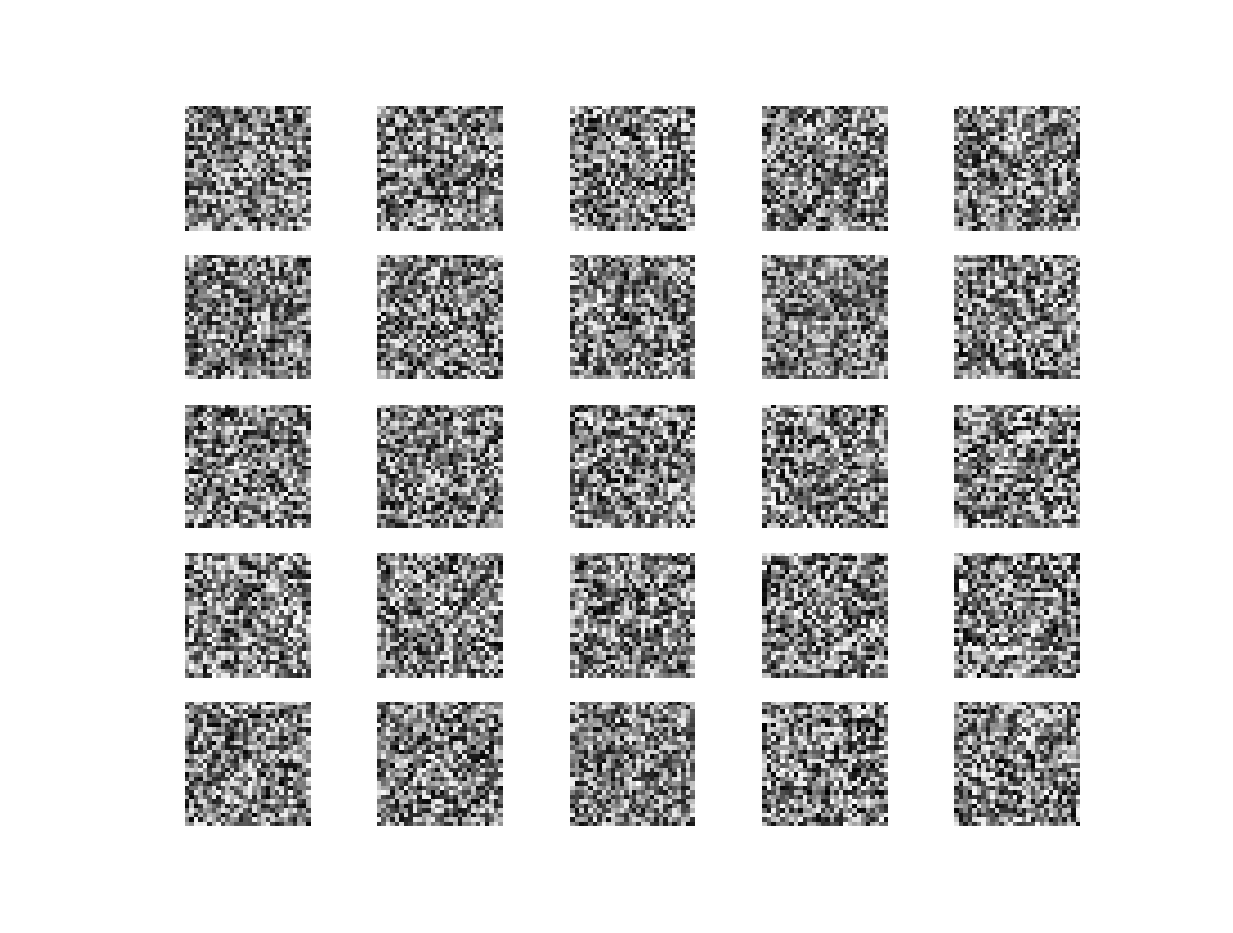
\includegraphics[width=0.4\textwidth]{assets/img/hidden_layer_analyze_mnist_image_nsamp70000_nh0.72.eps}
  \caption{識別性能が高い場合(中間層0.72)の重み}
  \label{fig:hidden-layer-analyze-img-0.72}
\end{figure}
%%%%%%%%%%%%%%%%%%%%%%%%%%%%%%%%%%%%%%%%%%%%%%%%%%%%%%%%
%%%%%%%%%%%%%%%%%%%%%%%%%%%%%%%%%%%%%%%%%%%%%%%%%%%%%%%%
%%%%%%%%%%%%%%%%%%%%%%%%%%%%%%%%%%%%%%%%%%%%%%%%%%%%%%%%
%%%%%%%%%%%%%%%%%%%%%%%%%%%%%%%%%%%%%%%%%%%%%%%%%%%%%%%%
%%%%%%%%%%%%%%%%%%%%%%%%%%%%%%%%%%%%%%%%%%%%%%%%%%%%%%%%


%%%%%%%%%%%%%%%%%%%%%%%%%%
% to insert bibliography %
%%%%%%%%%%%%%%%%%%%%%%%%%%
\begin{thebibliography}{9}
%   \bibitem{inv1} Samuel R.Buss,"Introduction to Inverse Kinematics with Jacobian Transpose,Pseudoinverse and Damped Least Squares methods"
  \bibitem{mnist} Yann LeCun, Corinna Cortes, Christopher J.C. Burges,
    ``MNIST handwritten digit database, Yann LeCun, Corinna Cortes and Chris Burges'',
    http://yann.lecun.com/exdb/mnist/
\end{thebibliography}

%%%%%%%%%%%%%%%%
% end document %
%%%%%%%%%%%%%%%%
\end{document}